\section{Perspektivering} \label{perspektivering}
I dette afsnit vil projektet perspektiveres for at kunne reflektere over de forskellige aspekter, der bør undersøges for at kunne skabe et færdigudviklet produkt, som kan anvendes af ALS-patienter. Systemet er udviklet til at kunne hjælpe ALS-patienter ved at aflaste deres muskler omkring knæet under en squat-øvelse. Der er ikke udviklet en prototype, der skal kunne muliggøre dette, hvorfor systemet skal videreudvikles, således det er anvendeligt uden at være til gene for brugeren. Et eksempel på dette fremgår af \autoref{fig:exoskelet}, hvor der ses et exoskelet påsat omkring knæet. Herudover vil det være fordelagtigt at sende en advarsel inden grænserne på $90^{\circ}$ og $180^{\circ}$ er overskredet i form af vibration eller lyd. Brugeren skal på nuværende tidspunkt selv starte og stoppe systemet, hvilket kan videreudvikles til en automatisk funktion, når brugeren udfører en bevægelse. 

\begin{figure}[H]
\centering
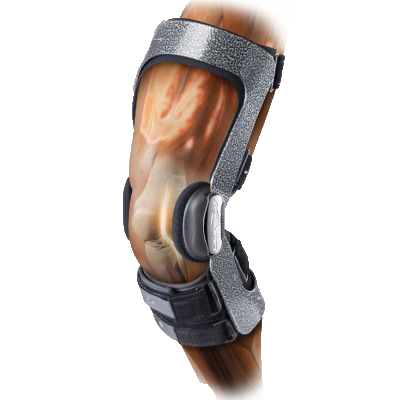
\includegraphics[width=0.5\textwidth]{figures/exoskelet}
\caption{en illustration af et exoskelet omkring knæet for at støtte den omkringliggende muskulator som hjælp til ALS-patienter \citep{djo}.}
\label{fig:exoskelet}
\end{figure}

\noindent
Herudover kan sammenhængen mellem de forskellige muskler i låret undersøges, således det vil være muligt at bevæge sig under $90^{\circ}$ og over $180^{\circ}$, da det vil være muligt at vurdere dette ud fra musklernes muskelaktivitet. Herudover kan det undersøges, hvordan mikrokontrolleren kan anvendes til opsætning af bluetooth kommunikation som det fremgår af det oprindelige design, da der på nuværende tidspunkt anvendes et gumstick til bluetooth kommunkation.(skal der referes til trådløs kommunikation??)

\subsection{Et ideelt system}
Systemet vil kunne videreudvikles, således det vil være muligt at anvende under gang for ALS-patienter, og derved støtte deres muskulatur, da det på nuværende tidspunkt kun er muligt at udføre en squat-øvelse. Systemet kan optimeres og forbedres på flere områder, da det har nogle begrænsninger, der betyder, at systemet ikke kan anvendes ved en vinkel under $90^{\circ}$ og over $180^{\circ}$. Dette skaber derfor nogle begrænsninger for brugerens bevægelighed. Systemet kan ligeledes udvikles til, at brugeren eksempelvis skal være i stand til at tænde og slukke systemet trådløst ved andvendelse af en mobiltelefon. En implementering i forhold til sikkerhed kan være en udvikling, hvor en alarm starter i tilfælde af, at brugeren mister balancen eller falder under gang. Dette vil kræve, at systemet ikke har nogle begrænsninger i forhold til vinklen. 




